% !TeX program = xelatex

\documentclass[
    aspectratio=169,
    handout,
]{beamer}

\usepackage{minted}
\usepackage{xcolor}
\usepackage{tcolorbox}
\usepackage{graphicx}
\usepackage{fontspec}
\usepackage{tabularray}

% allow to look for themes in another folder
% https://tex.stackexchange.com/a/284157/301699
\makeatletter
\def\beamer@calltheme#1#2#3{%
    \def\beamer@themelist{#2}
    \@for\beamer@themename:=\beamer@themelist\do
    {\usepackage[{#1}]{\beamer@themelocation/#3\beamer@themename}}}

\def\usefolder#1{
    \def\beamer@themelocation{#1}
}
\def\beamer@themelocation{}
\makeatother

\usefolder{..}
\usetheme{cexa-kokkos}

\AtBeginSection{
    \begin{frame}{Outline}
        \tableofcontents[currentsection, hideothersubsections]
    \end{frame}
}

\AtBeginSubsection{
    \begin{frame}{Outline}
        \tableofcontents[currentsection, currentsubsection]
    \end{frame}
}

\setminted{
    autogobble,
    fontsize=\small,
    bgcolor=lightgray,
    xleftmargin=0.5em,
    xrightmargin=0.5em,
    breaklines,
}

\NewTblrTheme{kokkostable}{
    \SetTblrInner{
        width=\linewidth,
        rowhead=1,
        rows={ht=\baselineskip},
        row{odd}={bg=lightgray},
        row{1}={bg=lightmain},
    }
}

\graphicspath{{../../images/}}

%Information to be included in the title page:
\title{Kokkos intermediate course}
\author{The CExA team}
\institute{CEA}
\date{\today}
\titlegraphic{%
    
\includegraphics[height=4em]{kokkos.png}%
    \hspace{1em}%
    
\includegraphics[height=4em]{cexa_logo.png}
}

% _____________________________________________________________________________

\begin{document}

\begin{frame}[plain]
    \titlepage
\end{frame}

% _____________________________________________________________________________

\begin{frame}{This course is open source}
    \begin{center}
        \githublink{\url{https://github.com/CExA-project/cexa-kokkos-tutorials}}
    \end{center}
\end{frame}

% _____________________________________________________________________________

\begin{frame}{Prerequisites}
    This course is intended for developers who have have followed the basic course of the tutorials

    \vspace{1em}

    \begin{block}{What you still need}
        \begin{itemize}
            \item Basic knowledge of C/C++
            \item Basic knowledge of parallel programming
            \item Basic knowledge of CMake
            \item Basic knowledge of a Linux environment
            \item Basic knowledge of Kokkos
        \end{itemize}
    \end{block}
\end{frame}

% _____________________________________________________________________________

\begin{frame}{Duration of the course}
    \begin{itemize}
        \item Course + practical work: full day
        \item Course + corrected exercise: half day
        \item Short version: 3 hours
    \end{itemize}
\end{frame}

\begin{frame}{Outline}
    \tableofcontents[hidesubsections]
\end{frame}

% _____________________________________________________________________________

\section{Profiling and debugging}

% _____________________________________________________________________________

\section{Subviews}

% _____________________________________________________________________________

\section{Atomics}

\begin{frame}[fragile]{Atomics - Race condition}
    \begin{columns}
        \begin{column}{0.4\linewidth}
            \begin{minted}{C++}
              Kokkos::View<double*>
                v("v", 2);
              // Init v with
              // v(0) = 4
              // v(1) = 5

              Kokkos::View<double> res;
              Kokkos::parallel_for(
                Kokkos::RangePolicy(0,2),
                KOKKOS_LAMBDA(int i) {
                  res() = res() + v(i);
                });
            \end{minted}
        \end{column}
        \begin{column}{0.6\linewidth}
          Even simple instruction like '\texttt{+}' are decomposed into several smaller assembly instructions:

          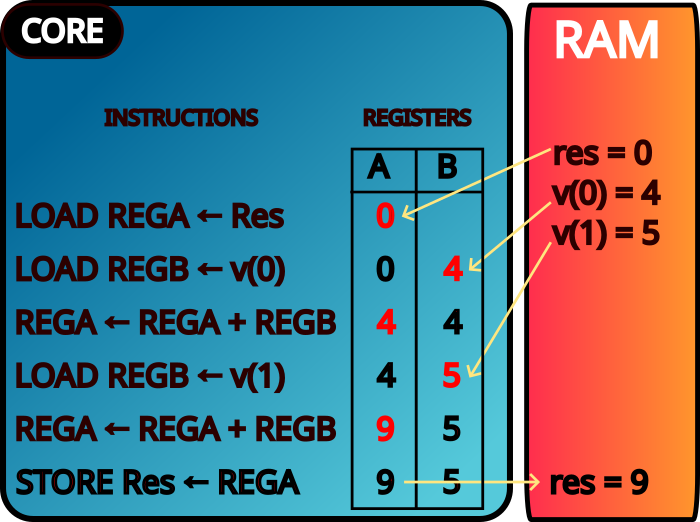
\includegraphics{race_condition1.png}
        \end{column}
    \end{columns}
\end{frame}

% Trainee could play with the following program to check that it really present a race condition:
%#include <iostream>
%#include <Kokkos_Core.hpp>
%
%int main(int argc, char *argv[]) {
%  Kokkos::initialize(argc, argv); 
%  {
%    const int N = 10000;
%    Kokkos::View<double*> v("v", N);
%    Kokkos::deep_copy(v, 4);
%
%    Kokkos::View<double> res("res", N);
%
%    Kokkos::parallel_for(Kokkos::RangePolicy(0, N),
%        KOKKOS_LAMBDA(int i) {
%        //Kokkos::atomic_add(&res(), v(i));
%        res() = res() + v(i);
%        });
%
%    double res_;
%
%    deep_copy(res_, res);
%
%    std::cout << "res_:" << res_ << std::endl;
%    std::cout << "4*N:" << 4*N << std::endl;
%  }
%  Kokkos::finalize();
%}

\begin{frame}[fragile]{Atomics - Race condition}
    \begin{columns}
        \begin{column}{0.4\linewidth}
            \begin{minted}{C++}
              Kokkos::View<double*>
                v("v", 2);
              // Init v with
              // v(0) = 4
              // v(1) = 5

              Kokkos::View<double> res;
              Kokkos::parallel_for(
                Kokkos::RangePolicy(0,2),
                KOKKOS_LAMBDA(int i) {
                  res() = res() + v(i);
                });
            \end{minted}
        \end{column}
        \begin{column}{0.6\linewidth}
          When several cores run in parallel, instructions can interleave and generate \structure{race conditions}:

          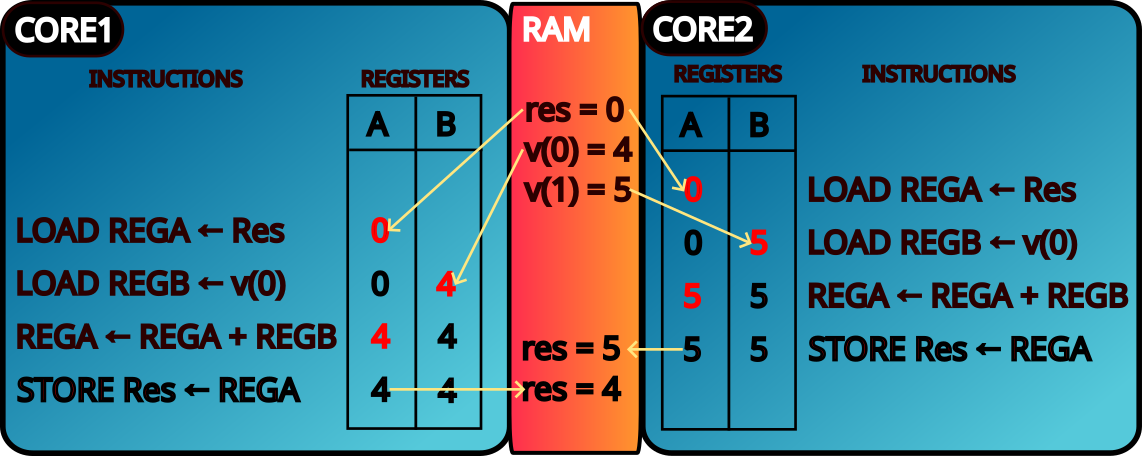
\includegraphics[width=1\textwidth]{race_condition2.png}
        \end{column}
    \end{columns}
\end{frame}

\begin{frame}[fragile]{Atomic Operations}
    \begin{columns}
        \begin{column}{0.4\linewidth}
            \begin{minted}{C++}
              Kokkos::View<double*>
                v("v", 2);
              // Init v with
              // v(0) = 4
              // v(1) = 5

              Kokkos::View<double> res;
              Kokkos::parallel_for(
                Kokkos::RangePolicy(0,2),
                KOKKOS_LAMBDA(int i) {
                  // res() += v(i)
                  Kokkos::atomic_add(
                    &res(), v(i));
                });
            \end{minted}
        \end{column}
        \begin{column}{0.5\linewidth}
          \texttt{atomic\_add} execute the \texttt{LOAD}, \texttt{STORE} and \texttt{ADD} in a single atomic step,
          guarantying the absence of race condition during the addition.
          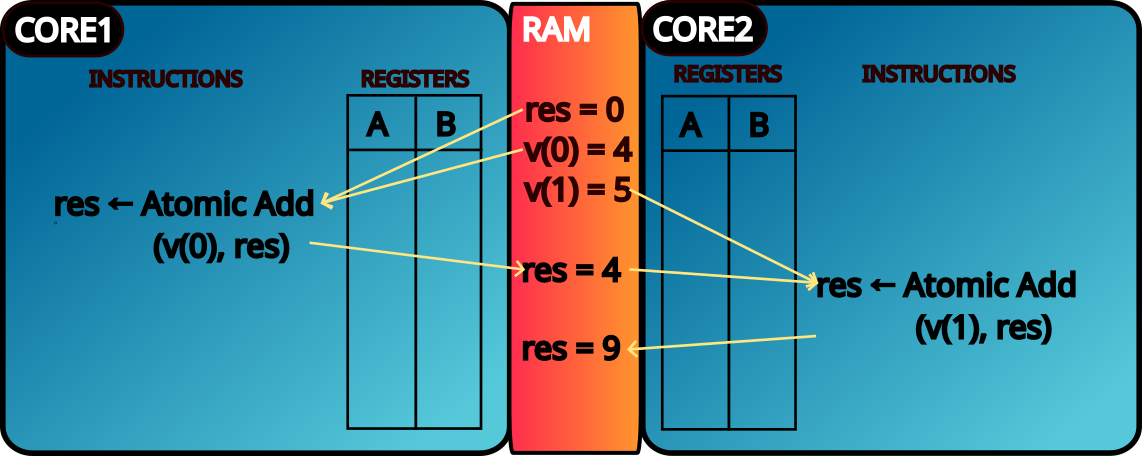
\includegraphics[width=1\textwidth]{race_condition3.png}
        \end{column}
    \end{columns}
  \pause
  Note that for this example, it would be better to use a \texttt{parallel\_reduce}.
\end{frame}

\begin{frame}[fragile]{Atomic operations}
  \begin{columns}
    \begin{column}{0.55\linewidth}
    \begin{tabular}{|l|c|}
      \hline
      Operation & Replaces \\
      \hline
      Kokkos::atomic\_add(\&x, y)    & x += y \\
      Kokkos::atomic\_and(\&x, y)    & x \&= y \\
      Kokkos::atomic\_dec(\&x)       & x-- \\
      Kokkos::atomic\_inc(\&x)       & x++ \\
      Kokkos::atomic\_lshift(\&x, y) & x = x << y \\
      Kokkos::atomic\_max(\&x, y)    & x = std::max(x, y) \\
      Kokkos::atomic\_min(\&x, y)    & x = std::min(x, y) \\
      Kokkos::atomic\_mod(\&x, y)    & x \%= y \\
      Kokkos::atomic\_nand(\&x, y)   & x = !(x \&\& y) \\
      Kokkos::atomic\_or(\&x, y)     & x |= y \\
      Kokkos::atomic\_rshift(\&x, y) & x = x >> y \\
      Kokkos::atomic\_sub(\&x, y)    & x -= y \\
      Kokkos::atomic\_store(\&x, y)  & x = y \\
      Kokkos::atomic\_xor(\&x, y)    & x \^{}= y \\
      \hline
    \end{tabular}
    \end{column}

      \begin{column}{0.35\linewidth}
        Other common operations are available with the format \texttt{Kokkos::atomic\_[op]}.
    \end{column}
  \end{columns}
\end{frame}

\begin{frame}[fragile]{Atomic operations - fetch}
    \begin{columns}
        \begin{column}{0.4\linewidth}
            \begin{minted}{C++}
              auto old_value =
                atomic_fetch_[op](
                  ptr_to_value,
                  update_value);

              auto new_value =
                atomic_[op]_fetch(
                  ptr_to_value,
                  update_value);
            \end{minted}
        \end{column}
        \begin{column}{0.6\linewidth}
          \texttt{atomic\_fetch\_[op]}:
          \begin{itemize}
            \item atomically performs the operation \texttt{[op]} with the operands \texttt{*ptr\_to\_value} and \texttt{update\_value},
            \item returns the value \texttt{*ptr\_to\_value} had \structure{before} the operation.
          \end{itemize}
          \texttt{atomic\_[op]\_fetch}:
          \begin{itemize}
            \item atomically performs the operation \texttt{[op]} with the operands \texttt{*ptr\_to\_value} and \texttt{update\_value},
            \item returns the value \texttt{*ptr\_to\_value} has \structure{after} the operation.
          \end{itemize}
        \end{column}
    \end{columns}
\end{frame}

\begin{frame}[fragile]{Atomic operations - Exchange}
    \begin{columns}
        \begin{column}{0.4\linewidth}
            \begin{minted}{C++}
              old_value =
                atomic_exchange(
                  ptr_to_value,
                  desired);

              old_value =
                atomic_compare_exchange(
                  ptr_to_value,
                  expected,
                  desired);
            \end{minted}
        \end{column}
        \begin{column}{0.6\linewidth}
          \texttt{atomic\_exchange}:
          \begin{itemize}
            \item atomically affects the value \texttt{desired} to \texttt{*ptr\_to\_value},
            \item returns the value \texttt{*ptr\_to\_value} had before the call.
          \end{itemize}
          \texttt{atomic\_compare\_exchange}:
          \begin{itemize}
            \item atomically affects the value \texttt{desired} to \texttt{*ptr\_to\_value}, \structure{if} the old value of \texttt{*ptr\_to\_value} was equal to \texttt{expected},
            \item returns the value \texttt{*ptr\_to\_value} had before the call, whether the exchange happened or not.
          \end{itemize}
        \end{column}
    \end{columns}
\end{frame}

\begin{frame}[fragile]{Atomic - Performances}
  Atomics can have a huge impact on performance: 
  \begin{itemize}
    \item the instruction itself is slower than the one it replaces,
    \item they may generates extra synchronisation points,
    \item they bypass and invalidate cache line.
  \end{itemize}

  => Atomics should be used with care and only when strictly necessary.\linebreak

  For some of your needs, more performant alternative exist, like \texttt{parallel\_reduce} or \texttt{Kokkos::ScatterView}.
\end{frame}

% _____________________________________________________________________________

\section{Layouts}

% _____________________________________________________________________________

\section{Scatter Views}

\end{document}
